\RequirePackage{plautopatch}  % pLaTeX または upLaTeX のとき
%\documentclass[uplatex,dvipdfmx,titlepage,a4j]{jsarticle}% upLaTeX のとき
\documentclass[dvipdfmx,titlepage,a4j]{jsarticle}  % pLaTeX のとき
\usepackage{listings,jvlisting}
\usepackage{amsmath,amssymb}
\usepackage{graphicx}
\usepackage[yen]{okuverb}
\usepackage{r04ec-exp}
\usepackage{here}
\usepackage{ascmac}
\usepackage{fancybox}
\usepackage{fancyvrb}
\usepackage{fancyhdr}
\usepackage{lastpage}

\fancypagestyle{foot}
{
\fancyhead[C]{トランジスタの増幅回路とR-L-C共振回路}
\fancyfoot[C]{\thepage / \pageref{LastPage}}
\renewcommand\headrulewidth{0.4pt}
}

\numberwithin{equation}{section}

%ここからソースコードの表示に関する設定
\lstset{
  language={C++},
  basicstyle={\ttfamily},
  identifierstyle={\small},
  commentstyle={\smallitshape},
  keywordstyle={\small\bfseries},
  ndkeywordstyle={\small},
  stringstyle={\small\ttfamily},
  frame={tb},
  tabsize={2},
  breaklines=true,
  columns=[l]{fullflexible},
  numbers=left,
  xrightmargin=0zw,
  xleftmargin=3zw,
  numberstyle={\scriptsize},
  stepnumber=1,
  numbersep=1zw,
  lineskip=-0.5ex
}

\renewcommand{\lstlistingname}{リスト}
%ここまでソースコードの表示に関する設定

\title{トランジスタの増幅回路とR-L-C共振回路}
% 学年・番号
\grade{4年42番}%
% 氏名
\author{鷲尾 優作}
% 班(後期は班に分かれて実験をする.そのときは,ここに班番号を記入する.)
\team{A1班}
% 提出日
\date{2022年6月16日}
% 実験日
\expdate{2022年5月26日,6月2日,6月9日}
% 共同実験者
% グループに分かれて実験をするテーマでは,グループメンバーの番号名前を書く.
\coauthor{}
%
%記載例:
%\coauthor{%
%  2番 & 新潟 花子\\
%  11番 & 三条 次郎}
%%

\begin{document}
\pagestyle{foot}

\maketitle

\section{背景・目的}
電子制御工学科4年前期(4年42番)のトランジスタの増幅回路とR-L-C共振回路実験について報告する.

半導体を用いて製造される能動素子であるトランジスタは, 「増幅作用」をもつが, 信号を増幅させる際,周辺回路の構成によって増幅特性に変化を生じる.
一方受動素子であるインダクタとコンデンサを用いる, LC回路は特定の周波数の信号を生成したり,複雑な信号から特定の周波数の信号だけを抽出するのに使用できる.

このレポートでは等価回路による理論値の算出,
バイポーラトランジスタを用いた増幅回路の実験, R-L-C回路共振回路の動作実験をそれぞれ行い,
理論値と実測値を比較しそれぞれの特性を確認した.

\section{トランジスタの増幅回路とその特性}
今回の実験では,エミッタ増幅回路をトランジスタの周辺回路として用いる.
トランジスタに直流バイアス成分を加え活性領域に動作点を設定し,
コンデンサ$C_1$を介して交流信号を重ねてトランジスタのベース端子に入力
増幅された交流信号をコレクタ端子に接続されたコンデンサ$C_2$を介して取り出す仕組みである.

図\ref{fig:tr}にエミッタ増幅回路を示す.

回路図上の各定数は以下のように設定した.

$R_1 = 22$ k$\Omega$, $R_2 = 100$ k$\Omega$, $R_3 = 2$ k$\Omega$, $R_4 = 10$ k$\Omega$,
$R_L = 10$ k$\Omega$, $C_1 = 0.1$ $\mu$F, $C_2 = 10$ $\mu$F, $E = 15$ V$R_1 = 22$ k$\Omega$, $R_2 = 100$ k$\Omega$, $R_3 = 2$ k$\Omega$, $R_4 = 10$ k$\Omega$,
$R_L = 10$ k$\Omega$, $C_1 = 0.1$ $\mu$F, $C_2 = 10$ $\mu$F, $E = 15$ V

\subsection{増幅回路の理論特性}
エミッタ増幅回路がどのような特性を示すか推定するため,電気的等価回路を作成し,
代表的な理論値を等価回路から導かれる計算式を用いて計算した.

\subsubsection{バイアス値}
トランジスタにおけるバイアス値は,交流信号を出力する際に基準となる電位の値であり,動作点を決定する重要な
パラメータである.バイアス値を導出する際には回路内の直流分のみを抽出した,「バイアス回路」を考える.

以下図 に実験で使用した回路をバイアス回路化したものを示す.

まず,$V_B$の電圧を導出する.
$I_{R2} \gg  I_B$であると仮定すると,$V_B$の電圧は式(\ref{eq:V_B})のように決定できる.

\begin{equation}
  V_B = \frac{R_1}{R_1 + R_2} \cdot E = \frac{22 \mathrm{[k\Omega]}}{22 \mathrm{[k\Omega]} + 100 \mathrm{[k\Omega]}} \cdot 15 \mathrm{[V]} \approx  2.7 \mathrm{[V]}
  \label{eq:V_B}
\end{equation}

次に$V_{E}$, $V_{C}$を導出する.
動作点を決定するために必要な各電圧$V_{E}$, $V_{C}$を求める計算式は以下のとおりとなる.

\begin{eqnarray}
  V_E &=& V_B - V_{BE} \\
  I_C &=& I_E = \frac{V_E}{R_3} \\
  V_C &=& E - R_4 I_C
\end{eqnarray}

$V_{BE}$を決定し,各電圧を導く.
使用するバイポーラトランジスタ2SC1815のデータシートより,$I_B - V_{BE}$特性表を図\ref{fig:ibvbe.png}に示す.
\begin{figure}[H]
  \centering
  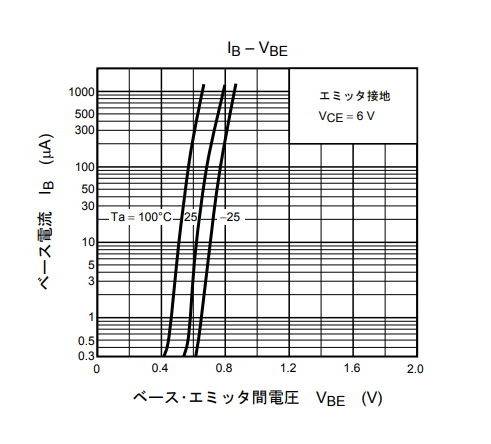
\includegraphics[width=9cm]{../2sc1815/ibvbe.png}
  \caption{2SC1815トランジスタの$I_B$-$V_{BE}$特性}
  \label{fig:ibvbe.png}
\end{figure}

特性表より,$V_{BE}\thickapprox 0.6 \mathrm{[V]}$と読み取ると,代入して各電圧は次のように求められる.
\begin{eqnarray}
  V_E &\approx& 2.7\mathrm{[V]} - 0.6\mathrm{[V]} = 2.1\mathrm{[V]}\\
  \label{eq:I_C}
  I_C &=& \frac{V_E}{R_3} = \frac{2.1\mathrm{[V]}}{2\mathrm{[k\Omega]}} = 1.05\mathrm{[mA]}\\
  V_C &=& E - R_4 I_C = 15\mathrm{[V]} - 10\mathrm{[k\Omega]} \cdot 1.05\mathrm{[mA]} = 4.5\mathrm{[V]}
\end{eqnarray}

\subsubsection{電圧利得}
電圧利得は,入力信号に対して出力信号の比が何dB上昇したかを表す.増幅回路そのものの性能を示すうえで重要な
パラメータである.電圧利得を算出するためには,まず結合コンデンサのインピーダンスを0とした交流分の等価回路を考える.

以下図 に実験で使用した回路の結合コンデンサのインピーダンスを0とした交流分の等価回路を示す.

ここで,
\begin{eqnarray}
  R_{12} &=& \frac{R_1 R_2}{R_1 + R_2} = \frac{22\mathrm{[k\Omega]} \cdot 100\mathrm{[k\Omega]}}{22\mathrm{[k\Omega]} + 100\mathrm{[k\Omega]}} = 18.0\mathrm{[k\Omega]} \\
  R_{4L} &=& \frac{R_4 R_L}{R_4 + R_L}= \frac{10\mathrm{[k\Omega]} \cdot 10\mathrm{[k\Omega]}}{10\mathrm{[k\Omega]} + 10\mathrm{[k\Omega]}} = 5.0\mathrm{[k\Omega]}
\end{eqnarray}
のように考えれば,簡易等価回路は図 のように簡単化できる.

電圧利得の理論値$G_V$は以下のような手順で導出できる.
\begin{eqnarray}
  V_i &=& h_{ie} I_b + (1+h_{fe})R_3 I_b \\
  V_o &=& h_{fe} I_b R_{4L} \\
  \left\lvert A_v \right\rvert &=& \frac{\left\lvert V_o \right\rvert}{\left\lvert V_i \right\rvert}
  = \frac{h_{fe} R_{4L}}{h_{ie} + (1+h_{fe})R_3} \\
  G_v &=& 20log_{10}(\left\lvert A_v \right\rvert)
\end{eqnarray}

導出に必要な直流電流増幅率$h_{fe}$,トランジスタの入力インピーダンス$h_{ie}$は,データシートより求める.
図\ref{fig:hic.png}に2SC1815のhパラメータ-$I_C$特性表を示す.

\begin{figure}[H]
  \centering
  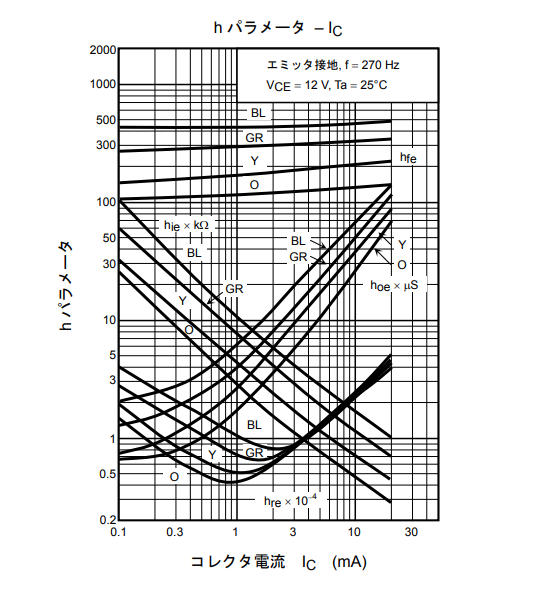
\includegraphics[width=9cm]{../2sc1815/hic.png}
  \caption{2SC1815トランジスタのhパラメータ-$I_C$特性}
  \label{fig:hic.png}
\end{figure}

式(\ref{eq:I_C})より,$I_C \thickapprox 1.0 \mathrm{[mA]}$であるから,
特性表より,$h_{fe} \thickapprox 160$,$h_ie \thickapprox 4.0 \mathrm{[k \Omega]}$と読み取れる.

これらの数値を用いて前式を解くと,電圧利得の理論値は以下のように導出できる.
\begin{eqnarray}
  V_i &=& h_{ie} I_b + (1+h_{fe})R_3 I_b \\
  V_o &=& h_{fe} I_b R_{4L} \\
  \left\lvert A_v \right\rvert &=& \frac{\left\lvert V_o \right\rvert}{\left\lvert V_i \right\rvert}
  = \frac{h_{fe} R_{4L}}{h_{ie} + (1+h_{fe})R_3} \\
  G_v &=& 20log_{10}(\left\lvert A_v \right\rvert)
\end{eqnarray}

\subsubsection{低域カットオフ周波数}
低域カットオフ周波数は,入力信号の周波数が減少した際に増幅が正常に行われなくなる現象において,その下限周波数の目安となる
パラメータである.低域カットオフは結合コンデンサ$C_1$によって生じるため,算出するためには$C_2$
を無視した簡易等価回路を考える.

以下図 に$C_2$を無視した簡易等価回路を示す.

ここで,
\begin{equation}
  R_{io} = \frac{R_{12} \{h_ie + ( 1 + h_fe)R_3\}}{R_{12} + \{h_ie + ( 1 + h_fe)R_3\}}
\end{equation}

のように考えれば,簡易等価回路は図 のように簡単化できる.

また,入力電圧を複素数空間に拡張すると,
\begin{equation}
  \dot{V} = \dot{V}_{ic} + \dot{V}_{io} = -j \frac{1}{\omega C_1} \dot{I}_i + R_{ic} \dot{I}_i
\end{equation}

低域カットオフ周波数の定義より,周波数低域において増幅率が3[dB]低下する点が$f_L$であるから,
このとき$\dot{V}_{io}$が$\dot{V}_{i}$の$\frac{1}{\sqrt{2}}$倍になることを利用すれば,
$\left\lvert \dot{V}_{ic} \right\rvert = \left\lvert \dot{V}_{io} \right\rvert$が成り立つ.

したがって,
\begin{eqnarray}
  \frac{1}{\omega_L C_1} &=& \frac{1}{2 \pi f_L C_1} = R_{io} \\
  f_L &=& \frac{1}{2 \pi C_1 R_{io}}
\end{eqnarray}

\subsubsection{入力インピーダンス}
回路全体の入力インピーダンスを算出する.
図 に結合コンデンサ$C_1$,$C_2$のインピーダンスを無視した簡易等価回路を示す.

入力側から見ると,入力インピーダンスは
\begin{equation}
  \dot{Z}_i = R_{io}
\end{equation}

\subsubsection{出力インピーダンス}
回路全体の出力インピーダンスを算出する.
入力インピーダンスの算出に使用した図 より

出力側から見ると,出力インピーダンスは
\begin{equation}
  \dot{Z}_o = R_4
\end{equation}

\subsubsection{出力波形の歪み}

\subsection{増幅回路の作成と実測}

\subsubsection{バイアス電圧の測定}

\subsubsection{電圧利得の測定}

\subsubsection{増幅率の周波数特性}

\subsubsection{入力インピーダンスの測定}

\subsubsection{出力インピーダンスの測定}

\subsubsection{増幅率の測定と波形歪みの観測}

\section{R-L-C共振回路とその特性}
R-L-C共振回路は,抵抗(Resistance),インダクタ(Inductance),キャパシタ(Capacitance)のそれぞれのインピーダンス特性を
利用し交流信号を入力として共振させることで周波数に対して特殊な応答を生じる回路である.

R-L-C共振回路は共振によって入力した周波数に対して全体のアドミッタンスが変化するアドミッタンス周波数特性を持つ.
アドミッタンスが最大となる入力周波数を$f_0$,最大値から$\frac{1}{\sqrt{2}}$倍となる周波数を$f_1$,$f_2$とすると.
アドミッタンス周波数特性は図 のようになる.

また,R-L-C共振回路ではアドミタンスの実部と虚部であるコンダクタンスとサセプタンスをXY成分としてプロットすると
円を描くことが知られている.この円を「アドミッタンスループ」と呼び,アドミッタンスループの各特徴点から有用な周波数や回路解析を行うことができる.
図 にアドミタンスループを示す.

\subsection{定数と理論特性}

\subsubsection{アドミッタンスと共振周波数}
図において角周波数$\omega$の信号を入力することを考える.
ここで回路全体のアドミッタンス$Z$は次式のようになるので,

\begin{equation}
  Z = R + j(\omega L - \frac{1}{\omega C})
\end{equation}

この時,複素アドミッタンス$\dot{Y}$とその大きさYは以下の式で求められる.

\begin{eqnarray}
  \dot{Y} &=& \frac{1}{Z} = \frac{1}{R + j(\omega L - \frac{1}{\omega C})} \\
  Y &=& \frac{1}{\dot{Y}} = \frac{1}{\sqrt{R + j(\omega L - \frac{1}{\omega C})}}
\end{eqnarray}

また,アドミッタンスが最大となる角共振周波数$\omega_0$,複素アドミッタンスの大きさ$Y_0$とすると,
複素アドミタンスの分母が最大となる時であるから,以下のように表せる.

\begin{eqnarray}
  \omega_0 L - \frac{1}{\omega_0 C} &=& 0 \\
  \omega_0 &=& \frac{1}{\sqrt{LC}} \\
  Y_0 &=& \frac{1}{\sqrt{R}}
\end{eqnarray}

\subsubsection{アドミッタンスループ}

複素パラメータ$R$(レジスタンス),$X$(リアクタンス),
$G$(コンダクタンス),$B$(サセプタンス)は複素インピーダンスと次式のような関係を持つ.

\begin{eqnarray}
  \dot{Z} = R + jX \\
  \dot{Y} = G + jB
\end{eqnarray}

2式の関係性を考えると,

\begin{eqnarray}
  R + jX &=& \frac{1}{G + jB} = \frac{G}{G^2 + B^2} -j\frac{B}{G^2 + B^2} \\
  R &=& \frac{G}{G^2 + B^2} \\
  0 &=& G^2 + B^2 - \frac{G}{R}
\end{eqnarray}

ここで,両辺に$(\frac{1}{2R})^2$を加算して式を整理すると,円の方程式が得られる.

\begin{eqnarray}
  (G - \frac{1}{2R})^2 + B^2 &=& (\frac{1}{2R})^2 \\
\end{eqnarray}

したがって,$G$(コンダクタンス),$B$(サセプタンス)を平面上にプロットしたとき描く円の
中心座標は,$(\frac{1}{2R}, 0)$,半径$\frac{1}{2R}$と定まる.

\subsubsection{品質係数Q値の算出}
Q値(Quality Factor)は,共振回路の共振のピークの鋭さを表す指標である.

R-L-C共振回路においては一般的に
\begin{eqnarray}
  Q = \frac{\omega_0 L}{R} = \frac{1}{\omega_0 CR}
\end{eqnarray}

となることが知られている.

振動の共振ピークの$sqrt{2}$倍となる入力周波数$\omega_2$,$\omega_1$とすると,
$\omega_2$,$\omega_1$におけるYの大きさは

\begin{eqnarray}
  Y &=& \frac{Y_0}{\sqrt{2}} = \frac{1}{\sqrt{2}R} \\
  Y &=& \frac{1}{\sqrt{R^2 + (\omega L - \frac{1}{\omega C})^2}}
\end{eqnarray}

$R$(レジスタンス)について整理すると

\begin{eqnarray}
  2R^2 &=& R^2 + (\omega L - \frac{1}{\omega C})^2 \\
  \pm R &=& (\omega L - \frac{1}{\omega C})
\end{eqnarray}

両辺に$\omega C$をかけて$\omega$を導くと

\begin{eqnarray}
  Lc \omega^2 + Rc\omega = 0\\
  \omega = \frac{\pm RC \pm \sqrt{(RC)^2 + 4LC}}{2LC}
\end{eqnarray}

$\omega_2 > \omega_1 > 0$であるから,

\begin{eqnarray}
  \omega_1 &=& \frac{-RC + \sqrt{(RC)^2 + 4LC}}{2LC} \\
  \omega_2 &=& \frac{+RC + \sqrt{(RC)^2 + 4LC}}{2LC} \\
  \omega_2 - \omega_1 &=& \frac{R}{L}
\end{eqnarray}

ここでQ値の定義を考えると

\begin{eqnarray}
  Q &=& \frac{\omega_0 L}{R} = \frac{\omega_0}{\omega2 - \omega_1}\\
\end{eqnarray}

となる.

\subsubsection{R, L, C値の算出方法}
R-L-Cの各定数が不明な際でも,アドミッタンスループを観測し$Y_0$,$\omega_0$,$\omega_1$,$\omega_2$を測定することで,
各定数成分を決定することができる.

\begin{eqnarray}
  R &=& \frac{1}{Y_0} \\
  L &=& \frac{Q}{\omega_0 Y_0} \\
  C &=& \frac{Y_0}{\omega_0 Q}
\end{eqnarray}

\subsection{R-L-C回路のアドミッタンス特性測定と定数の算出}

\subsubsection{アドミッタンス特性の測定}
R-L-C回路の特性評価を行うことができるLCRメーターを使用して入力周波数を自動で広範囲に可変し,アドミッタンス,
コンダクタンス,サセプタンスを測定することで,回路の周波数特性およびアドミッタンスループの観測を狙う.

\paragraph{アドミタンス周波数特性}

\paragraph{アドミッタンスループ特性}

\subsubsection{定数の算出}

\subsubsection{グラフの追記}

\section{課題}

\subsubsection{エミッタ接地,ベース接地,コレクタ接地の各増幅回路の特徴についてまとめよ.}

\subsubsection{共振回路の応用用途にはどのようなものがあるか調査し,それぞれについてまとめよ.}

\section{感想}

\begin{thebibliography}{99}
  \bibitem{umeda} 梅田 幹雄、実験テキスト「トランジスタの増幅回路とR-L-C共振回路」、(2022年)
\end{thebibliography}

\end{document}